\documentclass[12pt, twoside]{article}
\documentclass[12pt, twoside]{article}
\usepackage[letterpaper, margin=1in, headsep=0.2in]{geometry}
\setlength{\headheight}{0.6in}
%\usepackage[english]{babel}
\usepackage[utf8]{inputenc}
\usepackage{microtype}
\usepackage{amsmath}
\usepackage{amssymb}
%\usepackage{amsfonts}
\usepackage{siunitx} %units in math. eg 20\milli\meter
\usepackage{yhmath} % for arcs, overparenth command
\usepackage{tikz} %graphics
\usetikzlibrary{quotes, angles}
\usepackage{graphicx} %consider setting \graphicspath{{images/}}
\usepackage{parskip} %no paragraph indent
\usepackage{enumitem}
\usepackage{multicol}
\usepackage{venndiagram}

\usepackage{fancyhdr}
\pagestyle{fancy}
\fancyhf{}
\renewcommand{\headrulewidth}{0pt} % disable the underline of the header
\raggedbottom
\hfuzz=2mm %suppresses overfull box warnings

\usepackage{hyperref}
\usepackage{float}

\title{Algebra 2}
\author{Chris Huson}
\date{May 2024}

\fancyhead[LE]{\thepage}
\fancyhead[RO]{\thepage \\ Name: \hspace{3cm} \,\\}
\fancyhead[LO]{BECA / Huson / Algebra 2: Exponentials Jan 2023 Regents \\* May 2024}

\begin{document}

\subsubsection*{Jan 2023 Regents problems: Exponential functions}
\begin{enumerate}[itemsep=0.5cm]
\item The value of an automobile $t$ years after it was purchased is given by the function $V = 38,000(0.84)^t$. Which statement is true? %January 2023 Regents
\begin{enumerate}
    \item The value of the car increases 84\% each year.
    \item The value of the car decreases 84\% each year.
    \item The value of the car increases 16\% each year.
    \item The value of the car decreases 16\% each year.
\end{enumerate}

\item Which function represents exponential decay? %January 2023 Regents
\begin{enumerate}
    \item $\displaystyle p(x) = \left(\frac{1}{4}\right)^{-x}$
    \item $q(x) = 1.8^{-x}$
    \item $r(x) = 2.3^{2x}$
    \item $s(x) = 4^{\frac{x}{2}}$
\end{enumerate}

\item  %January 2023 Regents
Mia has a student loan that is in deferment, meaning that she does
not need to make payments right now. The balance of her loan
account during her deferment can be represented by the function
$f(x) = 35,000 (1.0325)^x$, where $x$ is the number of years since the
deferment began. If the bank decides to calculate her balance showing
a monthly growth rate, an approximately equivalent function would be
\begin{enumerate}
    \item $f(x) = 35,000 (1.0027)^{12x}$
    \item $\displaystyle f(x) = 35,000 (1.0027)^{\frac{x}{12}}$
    \item $f(x) = 35,000 (1.0325)^{12x}$
    \item $\displaystyle f(x) = 35,000 (1.0325)^{\frac{x}{12}}$
\end{enumerate}

\item To the \emph{nearest tenth}, the solution to the equation $4300e^{0.07x} -123 = 5000$ is %January 2023 Regents
\begin{enumerate}
    \item 1.1
    \item 2.5
    \item 6.3
    \item 68.5
\end{enumerate}

\newpage
\item For which approximate value(s) of $x$ will $\log(x+5) = |x-1|-3$? %January 2023 Regents
\begin{enumerate}
    \item $5,1$
    \item $-2.41, 0.41$
    \item $-2.41, 5$
    \item $5$, only
\end{enumerate}

\item What is the solution of $2(3^{x+4})=56$? %August 2023 Regents
\begin{enumerate}
    \item $x=\log_3 (28) -4$
    \item $x=-1$
    \item $x=\log(25) -4$
    \item $\displaystyle x=\frac{\log(56)}{\log(6)} -4$
\end{enumerate}

\item Consider the data in the table below. %2 points January 2023 Regents
\begin{center}
\begin{tabular}{|c|c|c|c|c|c|c|}
    \hline
$x$ & 1 & 2 & 3 & 4 & 5 & 6 \\
\hline
$y$ & 3.9 & 6 & 11 & 18.1 & 28 & 40.3 \\
\hline
\end{tabular}
\end{center}
State an exponential regression equation to model these data, rounding all values to the \emph{nearest thousandth}.

\newpage
\item Graph $c(x) = -9(3)^{x-4} + 2$ on the axes below. %4 points January 2023 Regents
    \begin{center}
    \begin{tikzpicture}[scale=0.7]
        \draw[thin,gray] (-10,-10) grid (10,10);
        \draw[thick,->] (-10,0) -- (10.5,0) node[below] {$x$};
        \draw[thick,->] (0,-10) -- (0,10.5) node[above] {$c(x)$};
        %\draw[<->,blue, thick, domain=-10.3:4.3, samples=100] plot (\x, {-9*(3^(\x-4)) + 2});
    \end{tikzpicture}
    \end{center}
    Describe the end behavior of $c(x)$ as $x$ approaches positive infinity. \\[2cm]
    Describe the end behavior of $c(x)$ as $x$ approaches negative infinity.

\newpage
\item Objects cool at different rates based on the formula below. %6 points January 2023 Regents
\begin{align*}
&T = (T_0 - T_R)e^{-rt} + T_R \\
&T_0: \text{initial temperature} \\
&T_R: \text{room temperature} \\
&r: \text{rate of cooling of the object} \\
&t: \text{time in minutes that the object cools to a temperature, T}
\end{align*}
Mark makes T-shirts using a hot press to transfer designs to the shirts. He removes a shirt from
a press that heats the shirt to $400^\circ$F. The rate of cooling for the shirt is 0.0735 and the room temperature is $75^\circ$F. Using this information, write an equation for the temperature of the shirt,
$T$, after $t$ minutes. \\[4cm]
Use the equation to find the temperature of the shirt, to the nearest degree, after five minutes. \\[4cm]
At the same time, Mark’s friend Jeanine removes a hoodie from a press that heats the hoodie to $450^\circ$F. After eight minutes, the hoodie measured $270^\circ$F. The room temperature is still $75^\circ$F. Determine the rate of cooling of the hoodie, to the \emph{nearest ten thousandth}. \\[4cm]
The T-shirt and hoodie were removed at the same time. Determine when the temperature will be the same, to the nearest minute

\newpage
\subsubsection*{Jan 2020 Regents problems: Exponential functions}

% January 2020 Regents - Problem 2
\item Chet has \$1200 invested in a bank account modeled by the function 
$P(n) = 1200(1.002)^n$, where $P(n)$ is the value of his account, in dollars, 
after $n$ months. Chet's debt is modeled by the function $Q(n) = 100n$, 
where $Q(n)$ is the value of debt, in dollars, after $n$ months. \\
After $n$ months, which function represents Chet's net worth, $R(n)$?
\begin{enumerate}
    \item $R(n) = 1200(1.002)^n + 100n$
    \item $R(n) = 1200(1.002)^{12n} + 100n$
    \item $R(n) = 1200(1.002)^n - 100n$
    \item $R(n) = 1200(1.002)^{12n} - 100n$
\end{enumerate}

% January 2020 Regents - Problem 4
\item Susan won \$2,000 and invested it into an account with an annual interest rate of 3.2\%. If her investment were compounded monthly, which expression best represents the value of her investment after $t$ years?
\begin{enumerate}
    \item $2000(1.003)^{12t}$
    \item $2000(1.032)^{\frac{t}{12}}$
    \item $2000(1.003)^{t}$
    \item $2000(1.032)^{12t}$
\end{enumerate}

% January 2020 Regents - Problem 12
\item The function $N(x) = 90(0.86)^x + 69$ can be used to predict the temperature of a cup of hot chocolate in degrees Fahrenheit after $x$ minutes. What is the approximate average rate of change of the temperature of the hot chocolate, in degrees per minute, over the interval $[0, 6]$?
\begin{enumerate}
    \item $-8.93$
    \item $-0.11$
    \item $0.11$
    \item $8.93$
\end{enumerate}

% January 2020 Regents - Problem 31
\item Biologists are studying a new bacterium. They create a culture with 100 of the bacteria and anticipate that the number of bacteria will double every 30 hours. Write an equation for the number of bacteria, $B$, in terms of the number of hours, $t$, since the experiment began.

% January 2020 Regents - Problem 36
\item The table below gives air pressures in kPa at selected altitudes above sea level measured in kilometers.
    \[
    \begin{array}{|c|c|c|c|c|c|c|c|}
    \hline
    x & \text{ (Altitude in km)} & 0 & 1 & 2 & 3 & 4 & 5 \\
    \hline
    y & \text{ (Air Pressure in kPa)} & 101 & 90 & 79 & 70 & 62 & 54 \\
    \hline
    \end{array}
    \]
Write an exponential regression equation that models these data rounding all values to the \emph{nearest thousandth}. \vspace{1cm}

Use this equation to algebraically determine the altitude, to the \emph{nearest hundredth} of a kilometer, when the air pressure is 29 kPa.

\newpage
\subsubsection*{August 2019 Regents problems: Exponential functions}

% August 2019 Regents - Problem 3
\item Perry invested in property that cost him \$1500. Five years later, it was worth \$3000, and 10 years from his original purchase, it was worth \$6000. Assuming the growth rate remains the same, which type of function could he create to find the value of his investment 30 years from his original purchase?
\begin{enumerate}
    \item exponential function
    \item linear function
    \item quadratic function
    \item trigonometric function
\end{enumerate}

% August 2019 Regents - Problem 17
\item If \$5000 is put into a savings account that pays 3.5\% interest compounded monthly, how much money, to the nearest ten cents, would be in that account after 6 years, assuming no money was added or withdrawn?
\begin{enumerate}
    \item \$5177.80
    \item \$5941.30
    \item \$6146.30
    \item \$6166.50
\end{enumerate}

% August 2019 Regents - Problem 18
\item The Fahrenheit temperature, $F(t)$, of a heated object at time $t$, in minutes, can be modeled by the function below. $F_s$ is the surrounding temperature, $F_0$ is the initial temperature of the object, and $k$ is a constant.
\[ F(t) = F_s + (F_0 - F_s)e^{-kt} \]
Coffee at a temperature of 195°F is poured into a container. The room temperature is kept at a constant 68°F and $k = 0.05$. Coffee is safe to drink when its temperature is, at most, 120°F. To the nearest minute, how long will it take until the coffee is safe to drink?
\begin{enumerate}
    \item 7
    \item 10
    \item 11
    \item 18
\end{enumerate}

% August 2019 Regents - Problem 24
\item A study of black bears in the Adirondacks reveals that their population can be represented by the function $P(t) = 3500(1.025)^t$, where $t$ is the number of years since the study began. Which function is correctly rewritten to reveal the monthly growth rate of the black bear population?
\begin{enumerate}
    \item $P(t) = 3500(1.00206)^{12t}$
    \item $P(t) = 3500(1.00206)^{t}$
    \item $P(t) = 3500(1.34489)^{\frac{t}{12}}$
    \item $P(t) = 3500(1.34489)^{12t}$
\end{enumerate}

% August 2019 Regents - Problem 33
\item A population of 950 bacteria grows continuously at a rate of 4.75\% per day.
\begin{enumerate}
    \item Write an exponential function, $N(t)$, that represents the bacterial population after $t$ days and explain the reason for your choice of base.
    \item Determine the bacterial population after 36 hours, to the nearest bacterium.
\end{enumerate}



\newpage
\subsubsection*{June 2019 Regents problems: Exponential functions}

% June 2019 Regents - Problem 5
\item A 7-year lease for office space states that the annual rent is \$85,000 for the first year and will increase by 6\% each additional year of the lease. What will the total rent expense be for the entire 7-year lease?
\begin{enumerate}
    \item \$42,809.63
    \item \$90,425.53
    \item \$595,000.00
    \item \$713,476.20
\end{enumerate}

% June 2019 Regents - Problem 10
\item Which situation could be modeled using a geometric sequence?
\begin{enumerate}
    \item A cell phone company charges \$30.00 per month for 2 gigabytes of data and \$12.50 for each additional gigabyte of data.
    \item The temperature in your car is 79°. You lower the temperature of your air conditioning by 2° every 3 minutes in order to find a comfortable temperature.
    \item David’s parents have set a limit of 50 minutes per week that he may play online games during the school year. However, they will increase his time by 5\% per week for the next ten weeks.
    \item Sarah has \$100.00 in her piggy bank and saves an additional \$15.00 each week.
\end{enumerate}

% June 2019 Regents - Problem 17
\item A savings account, \( S \), has an initial value of \$50. The account grows at a 2\% interest rate compounded \( n \) times per year, \( t \), according to the function below.
\[ S(t) = 50\left(1 + \frac{0.02}{n}\right)^{nt} \]
Which statement about the account is correct?
\begin{enumerate}
    \item As the value of \( n \) increases, the amount of interest per year decreases.
    \item As the value of \( n \) increases, the value of the account approaches the function \( S(t) = 50e^{0.02t} \).
    \item As the value of \( n \) decreases to one, the amount of interest per year increases.
    \item As the value of \( n \) decreases to one, the value of the account approaches the function \( S(t) = 50(1 + 0.02)^t \).
\end{enumerate}

% June 2019 Regents - Problem 20
\item Which table best represents an exponential relationship?
\begin{multicols}{4}
\begin{enumerate}

    \item 
    \[
    \begin{array}{|c|c|}
    \hline
    x & y \\
    \hline
    1 & 8 \\
    2 & 4 \\
    3 & 2 \\
    4 & 1 \\
    5 & \frac{1}{2} \\
    \hline
    \end{array}
    \]

    \item 
    \[
    \begin{array}{|c|c|}
    \hline
    x & y \\
    \hline
    8 & 0 \\
    4 & 1 \\
    0 & 2 \\
    -4 & 3 \\
    -8 & 4 \\
    \hline
    \end{array}
    \]

    \item 
    \[
    \begin{array}{|c|c|}
    \hline
    x & y \\
    \hline
    0 & 0 \\
    1 & 1 \\
    2 & 4 \\
    3 & 9 \\
    4 & 16 \\
    \hline
    \end{array}
    \]

    \item 
    \[
    \begin{array}{|c|c|}
    \hline
    x & y \\
    \hline
    1 & 1 \\
    2 & 8 \\
    3 & 27 \\
    4 & 64 \\
    5 & 125 \\
    \hline
    \end{array}
    \]
\end{enumerate}
\end{multicols}

% June 2019 Regents - Problem 24
\item Camryn puts \$400 into a savings account that earns 6\% annually. The amount in her account can be modeled by \( C(t) = 400(1.06)^t \) where \( t \) is the time in years. Which expression best approximates the amount of money in her account using a weekly growth rate?
\begin{enumerate}
    \item \( 400(1.001153846)^t \)
    \item \( 400(1.001153846)^{52t} \)
    \item \( 400(1.001121184)^t \)
    \item \( 400(1.001121184)^{52t} \)
\end{enumerate}

% June 2019 Regents - Problem 34
\item The half-life of a radioactive substance is 15 years.
\begin{enumerate}
    \item Write an equation that can be used to determine the amount, \( s(t) \), of 200 grams of this substance that remains after \( t \) years.
    \item Determine algebraically, to the nearest year, how long it will take for \(\frac{1}{10}\) of this substance to remain.
\end{enumerate}

% January 2019 Regents - Problem 6
\item Julia deposits \$2000 into a savings account that earns 4\% interest per year. The exponential function that models this savings account is \( y = 2000(1.04)^t \), where \( t \) is the time in years. Which equation correctly represents the amount of money in her savings account in terms of the monthly growth rate?
\begin{enumerate}
    \item \( y = 166.67(1.04)^{0.12t} \)
    \item \( y = 2000(1.01)^t \)
    \item \( y = 2000(1.0032737)^{12t} \)
    \item \( y = 166.67(1.0032737)^t \)
\end{enumerate}

% January 2019 Regents - Problem 17
\item If \( f(x) = a^x \) where \( a > 1 \), then the inverse of the function is
\begin{enumerate}
    \item \( f^{-1}(x) = \log x a \)
    \item \( f^{-1}(x) = \log_a x \)
    \item \( f^{-1}(x) = a^{\log x} \)
    \item \( f^{-1}(x) = x^{\log a} \)
\end{enumerate}

% January 2019 Regents - Problem 18
\item Kelly-Ann has \$20,000 to invest. She puts half of the money into an account that grows at an annual rate of 0.9\% compounded monthly. At the same time, she puts the other half of the money into an account that grows continuously at an annual rate of 0.8\%. Which function represents the value of Kelly-Ann’s investments after \( t \) years?
\begin{enumerate}
    \item \( f(t) = 10,000(1.9)^t + 10,000e^{0.8t} \)
    \item \( f(t) = 10,000(1.009)^t + 10,000e^{0.008t} \)
    \item \( f(t) = 10,000(1.075)^{12t} + 10,000e^{0.8t} \)
    \item \( f(t) = 10,000(1.00075)^{12t} + 10,000e^{0.008t} \)
\end{enumerate}

% January 2019 Regents - Problem 20
\item Sodium iodide-131, used to treat certain medical conditions, has a half-life of 1.8 hours. The data table below shows the amount of sodium iodide-131, rounded to the nearest thousandth, as the dose fades over time.
\[
\begin{array}{|c|c|c|c|c|c|}
\hline
\text{Number of Half Lives} & 1 & 2 & 3 & 4 & 5 \\
\hline
\text{Amount of Sodium Iodide-131} & 139.000 & 69.500 & 34.750 & 17.375 & 8.688 \\
\hline
\end{array}
\]
What approximate amount of sodium iodide-131 will remain in the body after 18 hours?
\begin{enumerate}
    \item 0.001
    \item 0.136
    \item 0.271
    \item 0.543
\end{enumerate}

% January 2019 Regents - Problem 37
\item Tony is evaluating his retirement savings. He currently has \$318,000 in his account, which earns an interest rate of 7\% compounded annually. He wants to determine how much he will have in the account in the future, even if he makes no additional contributions to the account.
    \begin{enumerate}
        \item Write a function, \( A(t) \), to represent the amount of money that will be in his account in \( t \) years.
        \item Graph \( A(t) \) where \( 0 \leq t \leq 20 \) on the set of axes below.
    \end{enumerate}
    \begin{center}
    
\begin{tikzpicture}[scale=0.7]
        \draw[thin,gray] (0,0) grid (20,20);
        \draw[thick,->] (0,0) -- (20.5,0) node[below] {$x$};
        \draw[thick,->] (0,0) -- (0,20.5) node[above] {$A(x)$};
    \end{tikzpicture}
    \end{center}

\end{enumerate}
\end{document}